\documentclass{article}
\usepackage{graphicx} % Required for inserting images
\usepackage[italian]{babel}
\usepackage[utf8]{inputenc}
\usepackage[T1]{fontenc}
\usepackage[sc,osf]{mathpazo}
\usepackage{amsmath, amssymb, mathtools}
\usepackage{textgreek}
\usepackage{nicefrac}
\usepackage{wrapfig}
\usepackage{subcaption}
\usepackage{capt-of}
\usepackage{cancel} % for strike-through
\usepackage{booktabs} % Linee orizzontali per tabelle ( \toprule \midrule \bottomrule )
\usepackage[font=small]{caption}
\usepackage[left=3.5cm, right=3.5cm]{geometry}
\usepackage[version=4,arrows=pgf-filled,textfontname=sffamily,mathfontname=mathsf]{mhchem}
\usepackage{footnote}
\usepackage{float}
\usepackage{threeparttable} % per tabelle con note a piè di pagina

\usepackage{siunitx}
\DeclareSIUnit\calorie{cal} % Definisco caloria
\sisetup{
  output-decimal-marker = {.},
  separate-uncertainty = true,
  table-align-uncertainty = true,
}
\newcommand{\interval}[3]{da \SI{#1}{#3} a \SI{#2}{#3}}

%Librerie per gestire elenchi (per bibliografia)
\usepackage{enumitem}
\usepackage{setspace}

\usepackage{csquotes} % dipendenza di biblatex
\usepackage[
  backend=biber,
  style=alphabetic,
  sorting=ynt
]{biblatex}
\addbibresource{bib.bib}
\AtBeginBibliography{\small}

\usepackage{comment}

%Comandi specifici per la relazione corrente
\newcommand{\ie}{\emph{i.e.}~}
\newcommand{\eg}{\emph{e.g.}~}
\newcommand{\therm}{\text{th}}
\newcommand{\paragrafo}[1]{\S\ref{#1}}

%Spazi tra tabelle e testo
\setlength{\textfloatsep}{1cm} % spazio tra tabelle e testo
\setlength{\floatsep}{1cm}      % spazio tra due tabelle consecutive

\usepackage[european]{circuitikz} % Oppure [american]
\usepackage{tikz}
\usepackage{pgfplots}
\pgfplotsset{compat=1.18}

\usepackage{xfp} % Pacchetto per calcoli matematici

% Comando automatico per calcolare Z-score e verificare compatibilità
\newcommand{\zcheck}[3]{%
  \edef\zval{\fpeval{round(abs((#2) - (#1)) / (#3), 2)}}%
  $Z = \zval \implies \ifnum\fpeval{\zval > 2}=1 \text{NO}\else \text{OK}\fi$%
}

% Comando per l'inserimento automatico dell'intera riga
% Sintassi: \riga{Grandezza}{V_teorico}{V_misurato}{Incertezza}
\newcommand{\riga}[4]{%
  #1 & #2 & #3 & #4 & \zcheck{#2}{#3}{#4} \\
}

\usepackage[colorlinks=true, linkcolor=red, citecolor=red, urlcolor=green]{hyperref} % per far si' che \ref reindirizzi al riferimento

\title{Esercitazione n.4+5}
\author{Lorenzo Girella, Aurora Lippi, Loris Masala}
\date{9 novembre 2026, Canale 2}

\begin{document}

\maketitle
\begin{abstract}
Nel seguente report vengono analizzate e descritte due esperienze di laboratorio, la prima si concentra su un sommatore non invertente a 3 ingressi, mentre la seconda su un filtro VCVS.
\end{abstract}

\tableofcontents

\section{Apparato Sperimentale}
La strumentazione utilizzata per la presa delle misure è costituita dai seguenti strumenti con relativi parametri caratteristici d'ingresso/uscita:
\begin{itemize}
    \item Multimetro digitale \textit{Fluke 45}: impedenza d'ingresso $R_{\text{in}} = 1\,\text{M}\Omega$ in parallelo a $C_{\text{in}} < 100\,\text{pF}$;
    \item Generatore di funzioni \textit{AFG-2225}: impedenza nominale di sorgente/uscita $Z_{\text{out}} = 50\,\Omega$;
    \item Oscilloscopio digitale a 2 canali \textit{Keysight EDUX1052G}: impedenza d'ingresso dei canali $R_{\text{in}} = 1\,\text{M}\Omega \parallel C_{\text{in}} \approx 16\,\text{pF}$;
    \item Alimentatore DC \textit{GPE-4323}: impedenza di uscita di valore trascurabile ($Z_{\text{out}} \approx 0.01\,\Omega$);
    \item Ponte LCR \textit{LXC100}.
\end{itemize}

\section{Mettere titolo}
\subsection{Misura del prodotto banda-guadagno, con TL082.}
Lo scopo di questa parte dell'analisi del circuito è comprendere l'andamento del guadagno del circuito a diverse configurazioni.
I componenti usati per la costruzione del circuito sono stati scelti considerando le caratteristiche del componente TL082, infatti a causa della sua natura di amplificatore per segnali non può erogare grandi correnti, di conseguenza vengono usate resistenze molto alte, dell'ordine dei \si{\kilo\ohm}.
Le misure con le relative incertezze delle resistenze usate nelle diverse configurazioni e le sinusoidi associate a quest'ultime vengono riportate nella seguente tabella:

\begin{table}[H]
    \centering
    \caption{Valori misurati delle resistenze con relative incertezze strumentali e tensioni applicate.}
    \label{tab:resistenze}
    \begin{tabular}{ccc}
        \toprule
        \textbf{Resistore} & \textbf{Resistenza misurata} & \textbf{Tensione ($v_{R'}$)} \\
        \midrule
        $R$    & \SI{1.0288 +- 0.0007}{\kilo\ohm} & \SI{100}{\milli\volt}$_{\text{pp}}$ \\
        $R'_1$ & \SI{4.672 +- 0.004}{\kilo\ohm}   & \SI{100}{\milli\volt}$_{\text{pp}}$ \\
        $R'_2$ & \SI{47.22 +- 0.04}{\kilo\ohm}    & \SI{100}{\milli\volt}$_{\text{pp}}$ \\
        $R'_3$ & \SI{100.06 +- 0.07}{\kilo\ohm}   & \SI{100}{\milli\volt}$_{\text{pp}}$ \\
        $R'_4$ & \SI{0.3288 +- 0.0004}{\mega\ohm} & \SI{50}{\milli\volt}$_{\text{pp}}$  \\
        \bottomrule
    \end{tabular}
\end{table}

Il circuito è stato montato sulla breadboard seguendo il seguente schema, inoltre affianco si allega una foto del circuito realizzato:

\begin{figure}[H]
    \centering
    \begin{subfigure}[b]{0.48\textwidth}
        \centering
        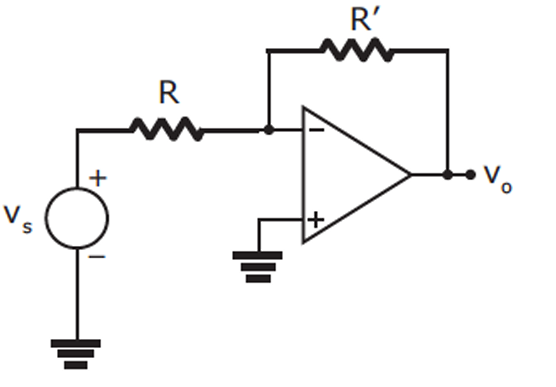
\includegraphics[width=\textwidth]{schemaCircuitoGuadagno-banda.png}
        \caption{Schema teorico del circuito.}
        \label{fig:schema_circuito}
    \end{subfigure}
    \hfill
    \begin{subfigure}[b]{0.48\textwidth}
        \centering
        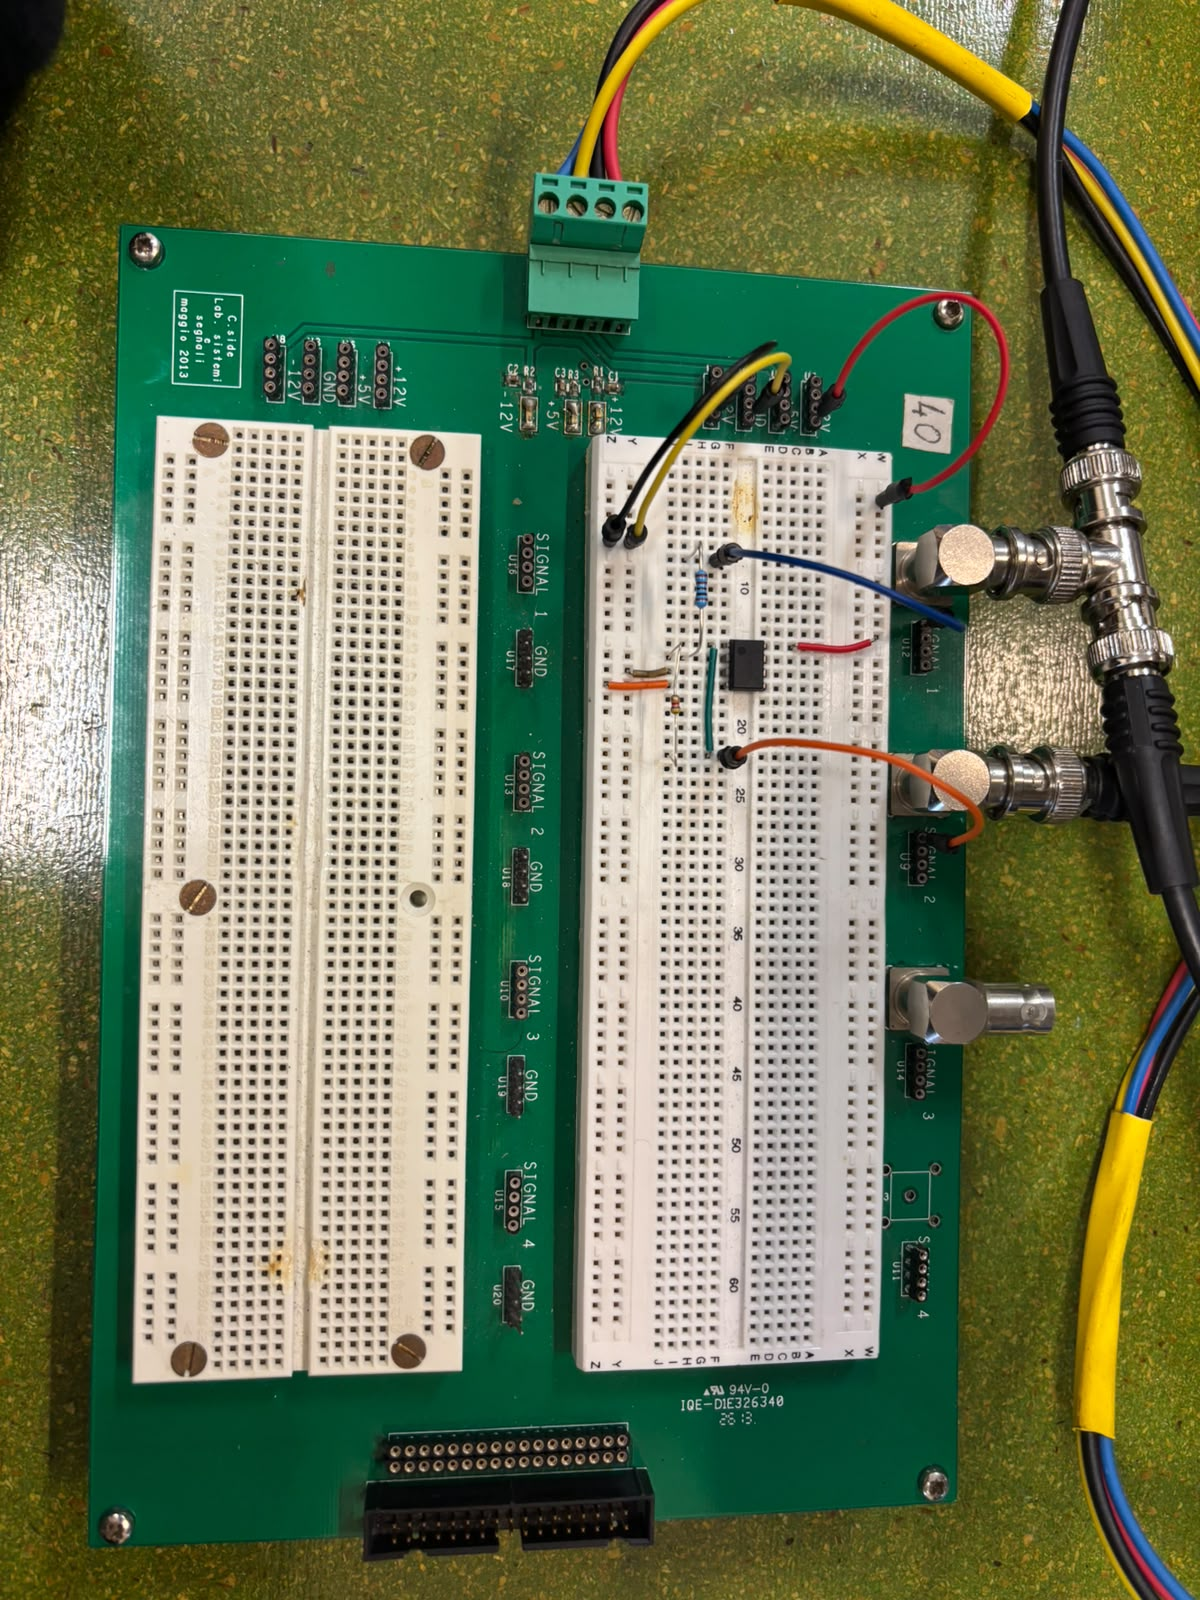
\includegraphics[angle=90, width=\textwidth]{circuitomontato.jpeg}
        \caption{Circuito montato sulla breadboard.}
        \label{fig:circuito_montato}
    \end{subfigure}
    \caption{Confronto tra lo schema teorico (a) e la realizzazione pratica sulla breadboard (b).}
    \label{fig:confronto_circuito}
\end{figure}

La breadboard è stata alimentata con una tensione di \SI{+12}{\volt} e \SI{-12}{\volt} in modo che la differenza delle tensioni sia inferiore a \SI{32}{\volt} in modo da evitare il cortocircuito del TL082, mentre le resistenze sono state collegate come da schema. 
Per ciascuna configurazione di resistenze è stata inviata una sinusoide con frequenza ad \SI{1}{\kilo\hertz} e con i valori di ampiezza riportati in Tabella~\ref{tab:resistenze}; successivamente è stata misurata l'ampiezza del valore in uscita $V_{\text{out}_{\text{pp}}}$ in modo da poter calcolare il guadagno del circuito in \si{\decibel} e il guadagno teorico grazie alle seguenti relazioni:
\begin{equation}
    A_{\max} = \frac{V_{\text{out}_{\text{pp}}}}{V_{\text{in}_{\text{pp}}}} \qquad \qquad A_{\max_{\text{dB}}} = 20 \cdot \log_{10}(A_{\max}) \qquad \qquad G=\frac{R'}{R}
\end{equation}
Dalle misure effettuate nelle diverse configurazioni di resistenze, si è potuto calcolare il guadagno teorico(G), che si riporta anche in decibel nella seguente tabella:
\begin{table}[H]
    \centering
    \caption{Valori teorici del guadagno a centro banda lineare ($|G|$) e in decibel ($G_{\text{dB}}$) per le quattro configurazioni del TL082.}
    \label{tab:guadagno_teorico}
    \begin{tabular}{ccc}
        \toprule
        \textbf{Configurazione} & \textbf{$|G|$} & \textbf{$G_{\text{dB}}$} \\
        \midrule
        $R'_1$ & \num{4.541} & \SI{13.143}{\decibel} \\
        $R'_2$ & \num{45.90} & \SI{33.236}{\decibel} \\
        $R'_3$ & \num{97.26} & \SI{39.759}{\decibel} \\
        $R'_4$ & \num{319.6} & \SI{50.092}{\decibel} \\
        \bottomrule
    \end{tabular}
\end{table}


\subsection{Misura della risposta in frequenza.}
Eseguendo un analisi della risposta in frequenza del circuito attraverso l'oscilloscopio e attraverso la presa di valori con l'uso dei cursori, si è potuto osservare come il guadagno del circuito vari al variare della frequenza del segnale in ingresso e costruire i diagrammi di bode per ogni configurazione di $R'$ e ricavare i valori del guadagno sperimentale a centro banda($A_{max}$), la frequenza di taglio($f_c=\frac{A_{max}}{\sqrt{3} }$) e il prodotto banda-guadagno($GBW=A_{max} \cdot f_c$).
Si riportano di seguito i grafici della risposta in frequenza per le quattro configurazioni del TL082 e il loro diagramma di bode:
\begin{table}[H]
    \centering
    \caption{Parametri sperimentali ricavati dal fit della risposta in frequenza per le quattro configurazioni del TL082: guadagno a centro banda ($A_0$), frequenza di taglio ($f_c$) e prodotto banda-guadagno ($\text{GBW}$).}
    \label{tab:risultati_fit}
    \begin{tabular}{cccc}
        \toprule
        \textbf{Configurazione} & \textbf{$A_0$} & \textbf{$f_c$} & \textbf{$\text{GBW}$} \\
        \midrule
        $R'_1$ & \num{4.70 +- 0.06}   & \SI{416 +- 10}{\kilo\hertz}     & \SI{1.96 +- 0.04}{\mega\hertz}  \\
        $R'_2$ & \num{47.65 +- 0.94}  & \SI{46.6 +- 1.3}{\kilo\hertz}   & \SI{2.22 +- 0.04}{\mega\hertz}  \\
        $R'_3$ & \num{100.8 +- 2.1}   & \SI{22.7 +- 0.6}{\kilo\hertz}   & \SI{2.28 +- 0.04}{\mega\hertz}  \\
        $R'_4$ & \num{326.10 +- 0.18} & \SI{7.800 +- 0.006}{\kilo\hertz} & \SI{2.540 +- 0.001}{\mega\hertz} \\
        \bottomrule
    \end{tabular}
\end{table}


\begin{figure}[H]
    \centering
        \centering
        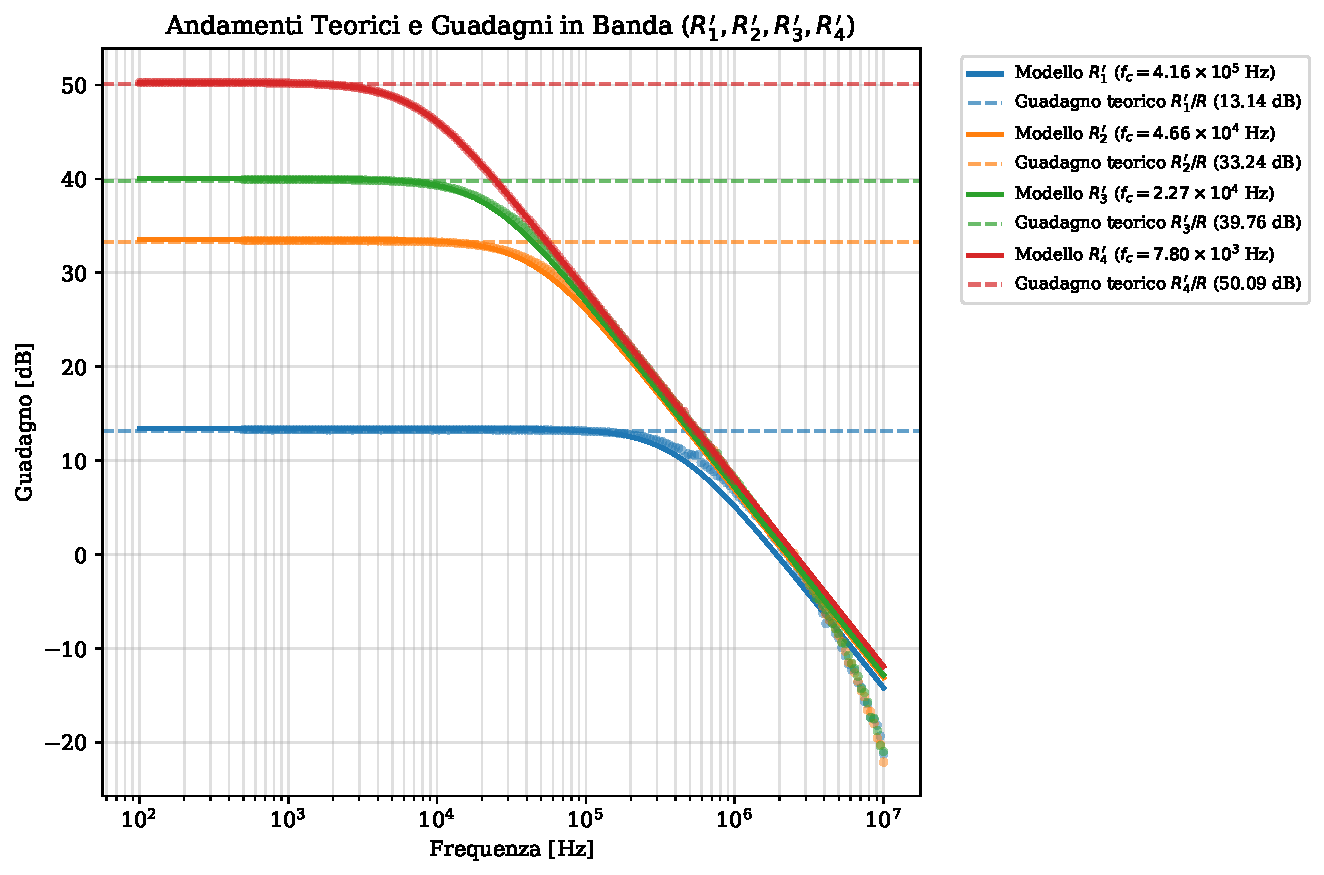
\includegraphics[width=0.75\textwidth]{bode_teorico_e_banda.pdf}
        \caption{Diagrammi di Bode per le quattro configurazioni di $R'$.}
    \end{figure}














\end{document}